%%%%%%%%%%%%%%%%%%%%%%%%%%%%%%%%%%%%%%%%%%%%%%%%%%%%%%%%%%%%%%%%%%%%%%%%%%%%%%%%%%%%%%%%%%
\documentclass[12pt]{article} %a4paper

\usepackage{graphicx} % to include pictures
\usepackage{subfig} % create subfigures within figures
\usepackage{pdflscape} % e.g. to rotate one page of the document
\usepackage{booktabs} % make better looking tabels with different line types and
%stuff
\usepackage[left=2.5cm,right=3cm,top=3cm,bottom=2.5cm]{geometry}
\usepackage{fancyhdr} % for pages with custom headers and footers
\usepackage[utf8]{inputenc}
\usepackage{float}
\usepackage{datetime}
\usepackage{natbib}
\bibliographystyle{unsrtnat}
\usepackage{setspace}
\usepackage{amsmath}
\usepackage{hyperref}
\usepackage{verbatim}
%\usepackage{pa}

\setlength{\parindent}{0.0in}
\setlength{\parskip}{1ex plus 0.5ex minus 0.2ex}
\mmddyyyydate
%%%%%%%%%%%%%%%%%%%%%%%%%%%%%%%%%%%%%%%%%%%%%%%%%%%%%%%%%%%%%%%%%%%%%%%%%%%%%%%%%%%%%%%%%%


\usepackage[english]{babel}															% English language/hyphenation
\usepackage[protrusion=true,expansion=true]{microtype}	
\usepackage{amsmath,amsfonts,amsthm} % Math packages
%\usepackage[pdftex]{graphicx}	
%\usepackage{verbatim}
\usepackage{url}
%\usepackage{float}


%%% Custom sectioning
\usepackage{sectsty}
\allsectionsfont{\centering \normalfont\scshape}


%%% Custom headers/footers (fancyhdr package)
\usepackage{fancyhdr}
\pagestyle{fancyplain}
\fancyhead{}											% No page header
\fancyfoot[L]{}											% Empty 
\fancyfoot[C]{}											% Empty
\fancyfoot[R]{\thepage}									% Pagenumbering
\renewcommand{\headrulewidth}{0pt}			% Remove header underlines
\renewcommand{\footrulewidth}{0pt}				% Remove footer underlines
\setlength{\headheight}{13.6pt}


%%% Equation and float numbering
\numberwithin{equation}{section}		% Equationnumbering: section.eq#
\numberwithin{figure}{section}			% Figurenumbering: section.fig#
\numberwithin{table}{section}				% Tablenumbering: section.tab#


%%% Maketitle metadata
\newcommand{\horrule}[1]{\rule{\linewidth}{#1}} 	% Horizontal rule


\title{
		%\vspace{-1in} 	
		\usefont{OT1}{bch}{b}{n}
		\normalfont \normalsize \textsc{Pennsylvania State University} \\ [25pt]
            \normalfont \normalsize \textsc{PLSC 597E} \\ [25pt]
		%\horrule{0.5pt} \\[0.2cm]
		\Large Replication Excercise: \textit{Self-Organizing Policy Networks: Risk, Partner, Selection, and Cooperation in Estuaries} \\
		%\horrule{2pt} \\[0.5cm]
}

\author{
		\normalfont 								\normalsize
        Joshua Snoke \\[-2pt]		\normalsize
}
\date{}


%%% Begin document
\begin{document}
\maketitle

\section*{Citation}
Berardo, Ramiro, and John T. Scholz. "Self-Organizing Policy Networks: Risk, Partner, Selection, and Cooperation in Estuaries." American Journal of Political Science 54, no. 3 (2010):632-649.

\section*{Data and Code}
\url{https://github.com/jsnoke/Replication-and-Extension}

\section{Background}
My replication study uses the paper "Self-Organizing Policy Networks: Risk, Partner, Selection, and Cooperation in Estuaries." by Berardo and Ramiro. This paper is of interest due to its use of two waves of longitudinal data with missingess in the second wave. The original paper did nothing beyond simple modal imputation or listwise deletion to account for this missingness.

The paper seeks to understand what attributes or network structures may cause nodes to create ties with one another. In this case, they consider water Estuaries and directed ties represent one group going to another group for advice. They also wish to model the level of trust between groups, measured at both time points. To do this they include a behavioral model to estimate different attribute effects on trust and simultaneously estimate these parameters alongside the network model. The two equations for the SAO model are as follows

\begin{equation}
f^{net}(x_{ij}) = \Sigma_k \beta_k^{net} s^{net}_{ijk}(x_{ij}) + \beta_k e_{ik}(x_i) + \beta_k a_{jk}(x_{j}) + \beta_k d_{ijk}(x_{ij}) + \epsilon^{net}
\end{equation}
\begin{equation}
f^{beh}(x) = \Sigma_k \beta_k e_{ik}(x_i) + \beta_k a_{jk}(x_{j}) + \epsilon^{beh}
\end{equation}

where $s_{ijk}$ represent network attributes, $e_{ik}$ represent ego (node forming tie) attributes, $a_{jk}$ represent alter (node being tied with) attributes, and $d_{ijk}$ represent similarity attributes.

I have obtained the complete data from the authors website, and have replicated most of the summary statistics and the Stochastic Actor Oriented model from the original paper. I have yet to be able to run the ERGM model or the MCMC method described due to a couple of issues with coding and missing data. The rest of the replication was successful, except there appears to be a slight discrepancy between the published result and the available data. Primarily this shows up in the second wave of the network data, where the data shows more missing nodes and different network statistics than reported.

\section{Replication}
This study replicated the simple network summary statistics and the Stochastic Actor Oriented model estimates across two waves of networks for cooperation in Estuaries. Extension involves ERGMs and considering alternative methods to deal with missing data prevelant in both the second wave and covariate data.

\subsection{Network Visuals}


\begin{figure}[!ht]
\centering
\begin{minipage}{.45\textwidth}
\centering
      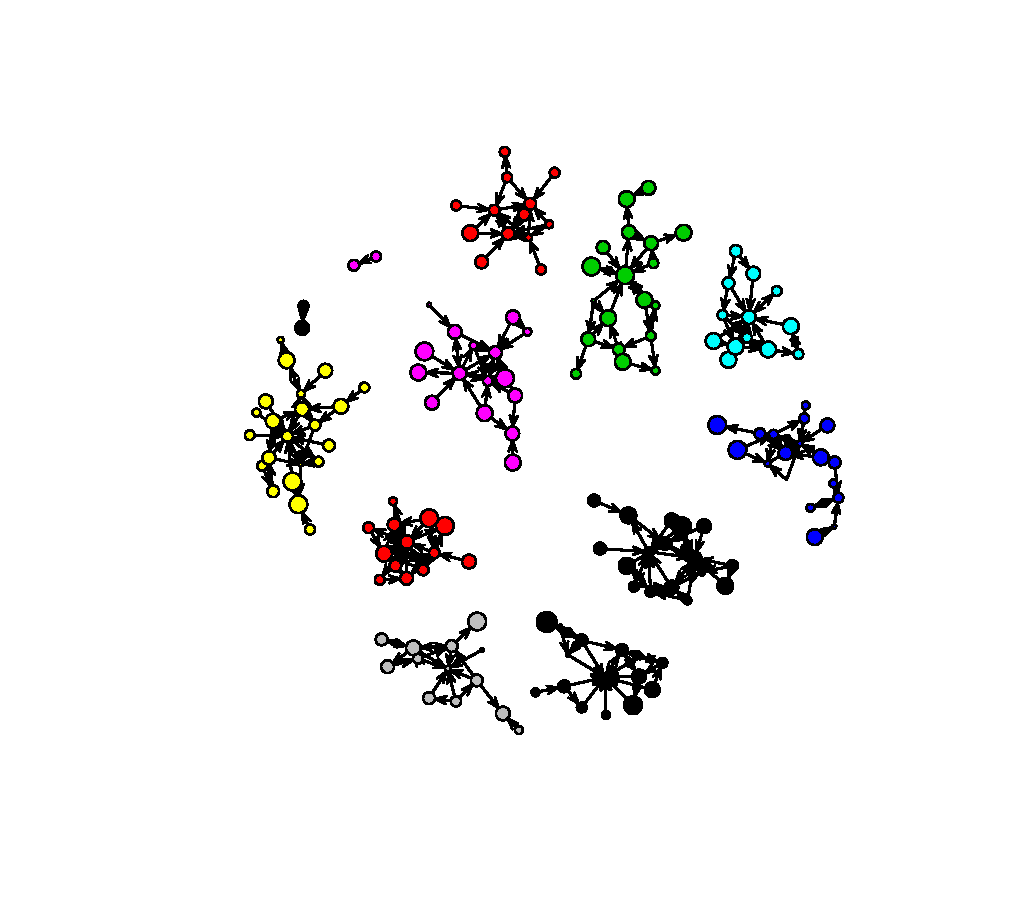
\includegraphics[width=\linewidth]{wave1plotT.pdf}
      \caption{Wave 1 network}\label{fig:x1}
\end{minipage}
\begin{minipage}{.45\textwidth}
\centering
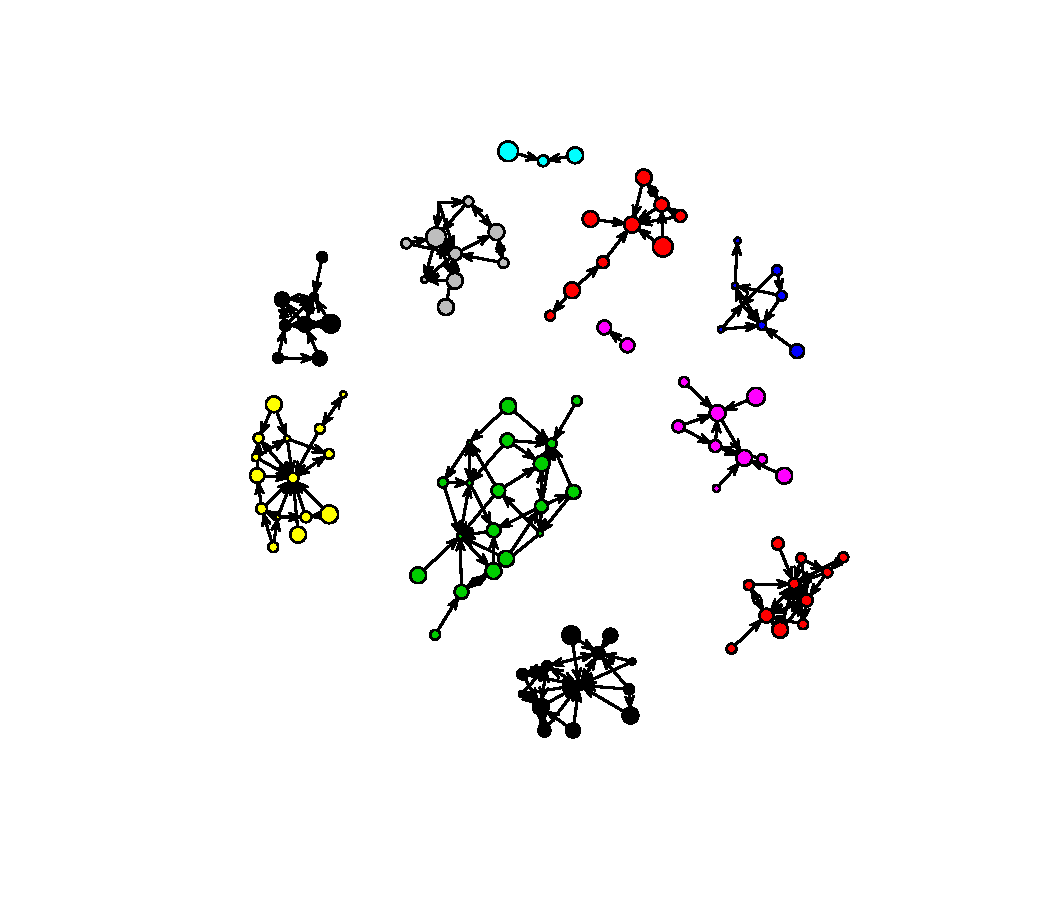
\includegraphics[width=\linewidth]{wave2plot.pdf}
      \caption{Wave 2 network}\label{fig:x2}
      \end{minipage}
\end{figure}


First, we simply visualize the first wave of the network data. We see as described and plotted in the paper that the network is directed and comprised of ten distinct communities. The nodes are colored by their Estuary group, and the node size is based on a covariate measured at each wave of how ``trustworthy'' a node was. Interestingly, there are also a number of isolates (not shown) which are not mentioned in the paper. In wave 2 we see that the network is substantially smaller, and the missingness is not even across Estuaries. This will lead to the extension of interest, namely imputing data.

\subsection{Network Exploration}
To further explore the network, we consider some network statistics. This is not part of the replication, as these exact statistics were not covered in the original paper, but it will help to better understand the data. Table \ref{tab07} gives results across the two waves for reciprocity, transitivity, betweenness centrality, and eigenvector centrality.

\begin{table}[!ht]
 	   \caption{\label{tab07} Network Statistics}
 	\centering
 	\begin{tabular}{lcc}
 		\hline
 		Statistic & Wave 1 & Wave 2 \\ 	
 		\hline
 		Reciprocity & 0.217 & 0.259 \\
 		Transitivity & 0.295 & 0.351 \\
 		Mean Normalized Betweenness Centrality & 0.047 & 0.095 \\
 		Mean Eigenvector Centrality & 0.027 & 0.052 \\
 		\hline
 	\end{tabular}
\end{table}

We see that all statistics increase for the second wave, which is interesting given its smaller number of nodes. Reciprocity and transitivity tell us that in the second wave, nodes are slightly more likely to recipricate ties and to tie with a third node if already tied to a second node which is tied to the third. Neither of the centrality measures are particularly high in either network. Figures \ref{fig:x3} and \ref{fig:x4} give histograms of the centralities across all nodes for the two waves. We see both have fairly long tail distributions.

\begin{figure}[!ht]
\centering
\begin{minipage}{.45\textwidth}
\centering
      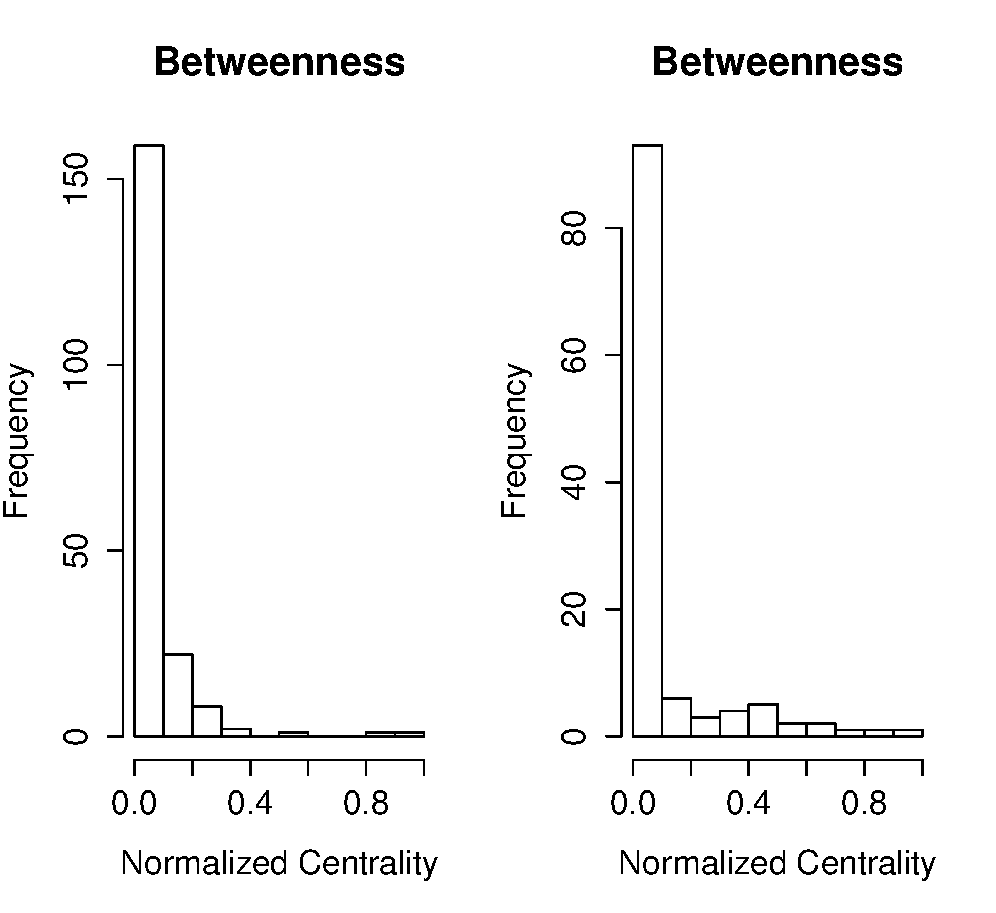
\includegraphics[width=\linewidth]{betweennessPlot.pdf}
      \caption{Betweenness Centrality Dist.}\label{fig:x3}
\end{minipage}
\begin{minipage}{.45\textwidth}
\centering
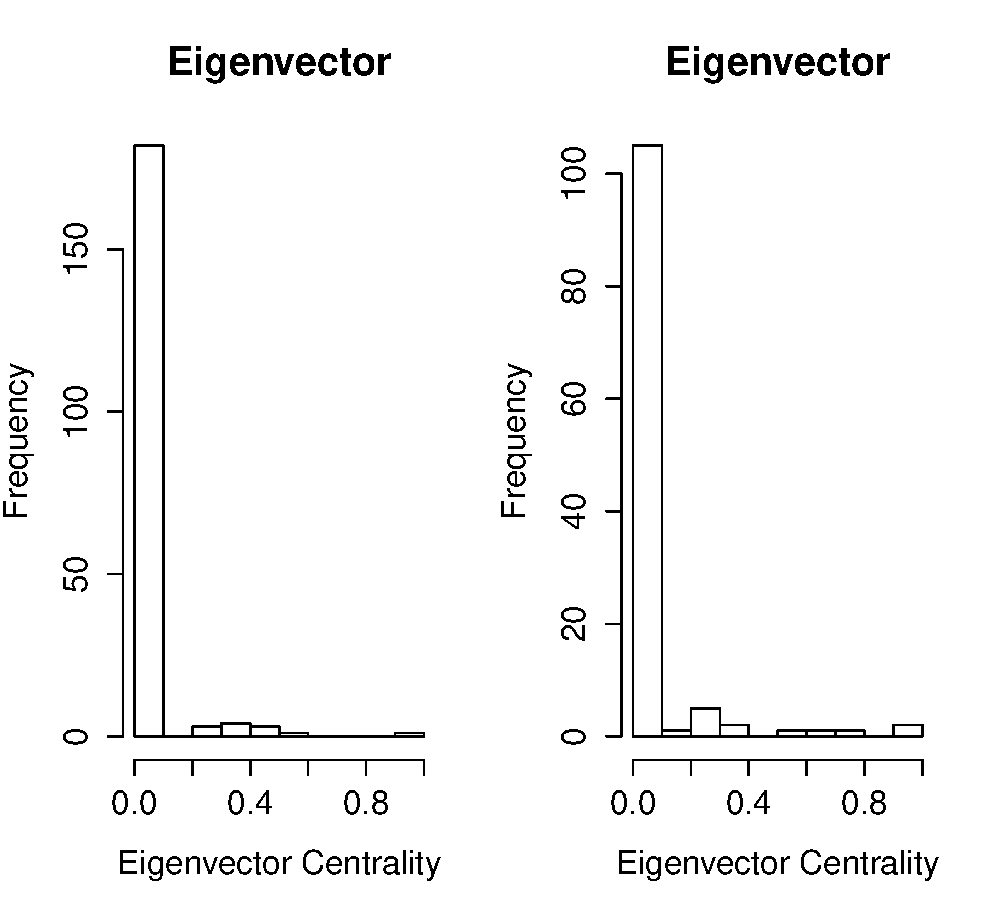
\includegraphics[width=\linewidth]{eigenvectorPlot.pdf}
      \caption{Eigenvector Centrality Dist.}\label{fig:x4}
      \end{minipage}
\end{figure}

\subsection{Descriptive Statistics}
Next, following Table A2 in the reference paper, we replicate the descriptive statistics for the two waves and the covariates. There were a number of difference between the replicated statistics and those given in the paper. These are bolded in the tables below.

\begin{table}[ht]
 	   \caption{\label{tab01} Covariate Statistics}
 	\centering
 	\begin{tabular}{lcccc}
 		\hline
 		Variable & Mean & SD & Min & Max \\ 	
 		\hline
 		Trust - wave 1 & 5.85 & 2.00 & 0 & 10 \\
 		Trust - wave 2 & 6.04 & 2.01 & 0 & 10 \\
 		Prodevelopment beliefs & 5.44 & \textbf{1.15} & 1 & 7 \\
 		Government actor & 0.49 & 0.50 & 0 & 1 \\
 		\hline
 	\end{tabular}
\end{table}

First, we see that the general covariate descriptive statistics in table \ref{tab01} are almost all exactly the same as published.

\begin{table}[ht]
 	   \caption{\label{tab02} Network Statistics}
 	\centering
 	\begin{tabular}{lcc}
 		\hline
 		Statistics & 1999 ($t_1$) & 2001 ($t_2$) \\ 	
 		\hline
 		Number of nodes & 194 & \textbf{118} \\
 		Number of networks & 10 & 10 \\
 		Average node in-degree & 1.43 & \textbf{1.69} \\
 		Number of total ties & 277 & \textbf{193} \\
 		Number of mutual dyads & 30 & \textbf{28} \\
 		Numer of asymmetric dyads & 217 & \textbf{143} \\
 		Number of transitive triplets & \textbf{72} & \textbf{51} \\
 		Number of out 2-stars & 205 & \textbf{116} \\
 		Number of in 2-stars & 533 & \textbf{398} \\
 		Number of 2-path & 505 & \textbf{318} \\
 		Missing data fraction & 0.00 & \textbf{0.39} \\
 		\hline
 	\end{tabular}
\end{table}

 The network statistics given in table \ref{tab02} on the other hand have a number of differences (bolded). First, the number of missing data points in the second wave is incorrect. 74 nodes are missing rather than 69, which also leads to all the network statistics being off. Secondly, there are a couple statistics in the first wave which are off, but I was not able to find exact definitions of how the original authors calculated these totals (transitive triplets, out 2-stars, in 2-stars), so it could be that I am simply calculating these differently. Lastly, it does not show up in these statistics, but a few nodes in the second wave have self-loops which by definition should be impossible. This leads me to believe the second data wave became somehow corrupted. This would explain the differences.

\begin{table}[ht]
 	   \caption{\label{tab03} Change in Links}
 	\centering
 	\begin{tabular}{lc}
 		\hline
 		Links & 1999 to 2001 \\ 	
 		\hline
 		0 $\rightarrow$ 0 & \textbf{35814} \\
 		0 $\rightarrow$ 1 & \textbf{152} \\
 		1 $\rightarrow$ 0 & 108 \\
 		1 $\rightarrow$ 1 & 89 \\
 		Missing & \textbf{1473} \\
 		\textit{note: undefined distances also given} & \\
 		\hline
 	\end{tabular}
 \end{table}

 \begin{table}[ht]
 	   \caption{\label{tab04} Change in Trust}
 	\centering
 	\begin{tabular}{lc}
 		\hline
 		Actor changes & 1999 to 2001 \\ 	
 		\hline
 		Constant & 37 \\
 		Up & \textbf{46} \\
 		Down & \textbf{42} \\
 		Total increase & \textbf{86} \\
 		Total decrease & \textbf{89} \\
 		Missing & 69 \\
 		\hline
 	\end{tabular}
 \end{table}

As exepected based on the previous table, the changes in links shown in table \ref{tab03} are slightly off from the published numbers. Curiously, the 1 to 0 and 1 to 1 changes were not corrupted. In the original paper, this table included some distance statistics but these were undefined and I was unable to replicate them.

Finally in table \ref{tab04} we look at the change in the trust covariate, since it was also measured at both waves. Here, the number of dropouts in the second wave is correct (69) unlike the network data. The number of nodes increasing or decreasing is off, only by 1, from the published results.

\subsection{Stochastic Actor Oriented Model}
The paper relies on one primary stochastic actor oriented (SAO) model. This is longitudinal and simultaneously models (i) a network equation for the choices made by nodes to form edges from the first wave to the second and (ii) a behavioral equation for the trust between nodes. The predictors in these models can be network attributes, actor or partner (referred to as ego and alter) covariates, or dyadic similarities across covariates. To fit this model requires a Markov Chain Monte Carlo (MCMC) estimation, switching between the equations to optimize across all parameters. Accordingly, results obtained here for replication will not be exact but should be similar to the published results. Models were estimated using the \emph{RSiena} package in \emph{R}. 

\begin{table}[ht]
 	   \caption{\label{tab05} SAO Model}
 	\centering
 	\begin{tabular}{lcc}
 		\hline
 		\textbf{Network Model - Partner Selection} & & \\
 		\hline
 		Variable & Coefficients & Standard Error \\
 		\hline
 		Average choice per actor & 4.85 & 0.49 \\
 		\textbf{Network structures} & & \\
 		Outdegree & -2.24 & 0.14 \\
 		Indegree & 0.21 & 0.02 \\
 		Reciprocity & 0.73 & 0.23 \\
 		Transitive triplets & 0.16 & 0.10 \\
 		\textbf{Ego attributes} & & \\
 		Generalized trust & -0.04 & 0.05 \\
 		Prodevelopment beliefs & 0.003 & 0.06 \\
 		Government actor & 0.003 & 0.14 \\
 		\textbf{Alter attributes} & & \\
 		Generalized trust & 0.006 & 0.05 \\
 		Prodevelopment beliefs & 0.02 & 0.06 \\
 		Government actor & 0.22 & 0.13 \\
 		\textbf{Dyadic Similarity} & & \\
 		Generalized trust & 0.16 & 0.82 \\
 		Prodevelopment beliefs & 0.61 & 0.46 \\
 		Government actor & 0.19 & 0.13 \\
 		\hline
 		& & \\
 		\hline
 		\textbf{Behavior Model - Partner Trust} & & \\
 		\hline
 		Variable & Coefficients & Standard Error \\
 		\hline
 		Average choices per actor & 6.85 & 1.20 \\
 		\textbf{Ego effects} & & \\
 		Trust in 1999 & 0.04 & 0.05 \\
 		Trust tendency & -0.006 & 0.02 \\
 		Prodevelopment beliefs & -0.06 & 0.05 \\
 		Government actor & 0.10 & 0.10 \\
 		\textbf{Alter effects} & & \\
 		Influence of Alters' trust & 4.12 & 2.22 \\
 		\hline
 	\end{tabular}
\end{table}

As these are simulated results the coefficients and standard errors will not be exactly the same, but generally they are very close to the published estimates. We can get a better idea also by looking at which variables are determined as significant. We see that there is one extra variable in our replication which is significant at the 0.01 level. Overall the smaller difference in model outcomes is good considering the data used for replication is not exactly the same as reported (based on the descriptive statistics). Note that p-values are obtained from running five simulations and performing a meta-analysis to determine significance among any simulation. They do not state in the published paper how they obtain p-values.

\begin{table}[!ht]
 	   \caption{\label{tab06} Significant Coefficients at 0.01 level}
 	\centering
 	\begin{tabular}{lc}
 		\hline
 		Published results & \textit{Outdegree, Indegree, Reciprocity, Influence of Alters' trust} \\ 	
 		\hline
 		\hline
 		Replicated results & \textit{Outdegree, Indegree, Reciprocity,} \\
 		& \textit{\textbf{(Alter) Government Actor}, Influence of Alters' trust} \\
 		\hline
 	\end{tabular}
\end{table}

\subsection{ERGM Models}
Discussion of ERGM models fit in paper, which are not replicable.

\section{Extension}
Two primary extensions.

\begin{enumerate}
\item Respecifying ERGM models in order to allow for estimating of ERGM models.
\item Considering different imputations.
\end{enumerate}

\subsection{Respecification of ERGM Models}
\begin{itemize}
\item Set constraints for outdegree following stated survey design.
\item Use previous wave as predictor of ties.
\item Implement a "build-up" modeling approach. First fitting an ERGM with appropriate structural statistics and then fitting successive models that add layers of the authors hypotheses. The goal will be to assess at what layer the model is best.
\end{itemize}

\subsection{Data Imputation Models}
\begin{itemize}
\item Modal imputation.
\item Carry forward imputation.
\item MPLE imputation - as a multiple imputation task
\item MPLE imputation - as a classification task
\end{itemize}

\subsection{Results - SAO models and new ERGMs with imputation}

\section{Conclusions}



\end{document}


